\documentclass[]{article}
\usepackage{lmodern}
\usepackage{amssymb,amsmath}
\usepackage{ifxetex,ifluatex}
\usepackage{fixltx2e} % provides \textsubscript
\ifnum 0\ifxetex 1\fi\ifluatex 1\fi=0 % if pdftex
  \usepackage[T1]{fontenc}
  \usepackage[utf8]{inputenc}
\else % if luatex or xelatex
  \ifxetex
    \usepackage{mathspec}
  \else
    \usepackage{fontspec}
  \fi
  \defaultfontfeatures{Ligatures=TeX,Scale=MatchLowercase}
\fi
% use upquote if available, for straight quotes in verbatim environments
\IfFileExists{upquote.sty}{\usepackage{upquote}}{}
% use microtype if available
\IfFileExists{microtype.sty}{%
\usepackage{microtype}
\UseMicrotypeSet[protrusion]{basicmath} % disable protrusion for tt fonts
}{}
\usepackage[margin=1in]{geometry}
\usepackage{hyperref}
\hypersetup{unicode=true,
            pdftitle={SSA 200 Course Evaluation},
            pdfauthor={Anna Tucker},
            pdfborder={0 0 0},
            breaklinks=true}
\urlstyle{same}  % don't use monospace font for urls
\usepackage{graphicx,grffile}
\makeatletter
\def\maxwidth{\ifdim\Gin@nat@width>\linewidth\linewidth\else\Gin@nat@width\fi}
\def\maxheight{\ifdim\Gin@nat@height>\textheight\textheight\else\Gin@nat@height\fi}
\makeatother
% Scale images if necessary, so that they will not overflow the page
% margins by default, and it is still possible to overwrite the defaults
% using explicit options in \includegraphics[width, height, ...]{}
\setkeys{Gin}{width=\maxwidth,height=\maxheight,keepaspectratio}
\IfFileExists{parskip.sty}{%
\usepackage{parskip}
}{% else
\setlength{\parindent}{0pt}
\setlength{\parskip}{6pt plus 2pt minus 1pt}
}
\setlength{\emergencystretch}{3em}  % prevent overfull lines
\providecommand{\tightlist}{%
  \setlength{\itemsep}{0pt}\setlength{\parskip}{0pt}}
\setcounter{secnumdepth}{0}
% Redefines (sub)paragraphs to behave more like sections
\ifx\paragraph\undefined\else
\let\oldparagraph\paragraph
\renewcommand{\paragraph}[1]{\oldparagraph{#1}\mbox{}}
\fi
\ifx\subparagraph\undefined\else
\let\oldsubparagraph\subparagraph
\renewcommand{\subparagraph}[1]{\oldsubparagraph{#1}\mbox{}}
\fi

%%% Use protect on footnotes to avoid problems with footnotes in titles
\let\rmarkdownfootnote\footnote%
\def\footnote{\protect\rmarkdownfootnote}

%%% Change title format to be more compact
\usepackage{titling}

% Create subtitle command for use in maketitle
\newcommand{\subtitle}[1]{
  \posttitle{
    \begin{center}\large#1\end{center}
    }
}

\setlength{\droptitle}{-2em}

  \title{SSA 200 Course Evaluation}
    \pretitle{\vspace{\droptitle}\centering\huge}
  \posttitle{\par}
    \author{Anna Tucker}
    \preauthor{\centering\large\emph}
  \postauthor{\par}
      \predate{\centering\large\emph}
  \postdate{\par}
    \date{October 29, 2018}

\usepackage{booktabs}
\usepackage{longtable}
\usepackage{array}
\usepackage{multirow}
\usepackage[table]{xcolor}
\usepackage{wrapfig}
\usepackage{float}
\usepackage{colortbl}
\usepackage{pdflscape}
\usepackage{tabu}
\usepackage{threeparttable}
\usepackage{threeparttablex}
\usepackage[normalem]{ulem}
\usepackage{makecell}

\begin{document}
\maketitle

\hypertarget{pre--and-post-class-assessment}{%
\subsubsection{Pre- and post-class
assessment}\label{pre--and-post-class-assessment}}

We asked four multiple choice questions before and after the course to
assess both baseline understanding and our effectiveness at
communicating some key ideas.

\hypertarget{questions}{%
\paragraph{Questions}\label{questions}}

\emph{The correct answers are in bold}

\begin{enumerate}
\def\labelenumi{\arabic{enumi}.}
\tightlist
\item
  What is a model?\\
\end{enumerate}

\begin{enumerate}
\def\labelenumi{\alph{enumi}.}
\tightlist
\item
  Someone who walks in fashion shows and is photographed a lot.\\
\item
  A mathematical equation.\\
  \textbf{c. A simplified representation of reality.}\\
\item
  A computer program used to predict future events.
\end{enumerate}

\begin{enumerate}
\def\labelenumi{\arabic{enumi}.}
\setcounter{enumi}{1}
\tightlist
\item
  What information does a regression coefficient tell you?\\
  \textbf{a. It quantifies the relationship between a predictor variable
  and a response variable.}\\
\end{enumerate}

\begin{enumerate}
\def\labelenumi{\alph{enumi}.}
\setcounter{enumi}{1}
\tightlist
\item
  It describes the correlation between two predictor variables in the
  model.\\
\item
  It tells you the probability that a covariate is an important
  predictor of the response variable.\\
\item
  It tells you how close the observed value is to the mean.
\end{enumerate}

\begin{enumerate}
\def\labelenumi{\arabic{enumi}.}
\setcounter{enumi}{2}
\tightlist
\item
  What types of uncertainty can we resolve using statistical models?\\
\end{enumerate}

\begin{enumerate}
\def\labelenumi{\alph{enumi}.}
\tightlist
\item
  Demographic stochasticity and observational uncertainty\\
  \textbf{b. Observational uncertainty and ecological uncertainty}\\
\item
  Partial controllability and environmental stochasticity\\
\item
  Environmental stochasticity and demographic stochasticity
\end{enumerate}

\begin{enumerate}
\def\labelenumi{\arabic{enumi}.}
\setcounter{enumi}{3}
\tightlist
\item
  Which of the following statements is a correct interpretation of the
  population projection below?\\
  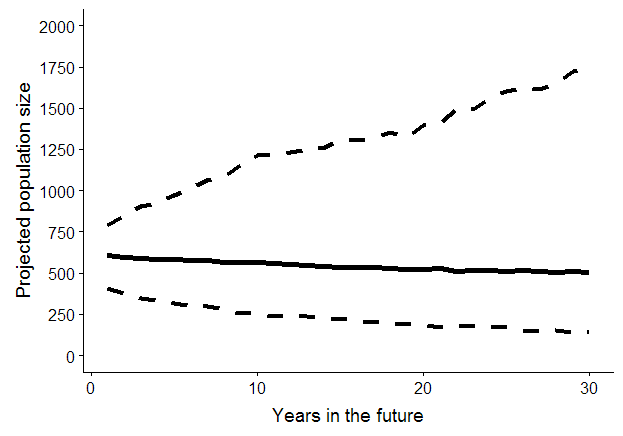
\includegraphics{img/pop-trend.png}
\end{enumerate}

\begin{enumerate}
\def\labelenumi{\alph{enumi}.}
\tightlist
\item
  This population has high resiliency.\\
\item
  This population will most likely be extinct in 30 years.\\
  \emph{c. This population will most likely remain stable for the next
  30 years.}\\
\item
  It is more likely than not that there will be at least 1000
  individuals in the population in 30 years.
\end{enumerate}

\hypertarget{reponses}{%
\paragraph{Reponses}\label{reponses}}

\begin{center}\includegraphics{eval_Oct2018_files/figure-latex/unnamed-chunk-2-1} \end{center}

\begin{verbatim}
## # A tibble: 2 x 2
##   type       `Average score`
##   <fct>                <dbl>
## 1 Pre-class            0.516
## 2 Post-class           0.641
\end{verbatim}

Overall the assessment scores improved after the class, with the average
increasing from 0.516 before the course to 0.641 after. The overall
distribution of scores shifted higher.

\begin{center}\includegraphics{eval_Oct2018_files/figure-latex/unnamed-chunk-4-1} \end{center}

The proportion of correct answer improved for all questions except for
question 1, which most students answered correctly before the class as
well.

\hypertarget{course-evaluations}{%
\paragraph{Course evaluations}\label{course-evaluations}}

We asked students to complete an anonymous course evaluation via Google
Forms.

\begin{verbatim}
## Sheet successfully identified: "SSA 200 Course Evaluation (Responses)"
\end{verbatim}

\begin{verbatim}
## Accessing worksheet titled 'Form Responses 1'.
\end{verbatim}

\begin{verbatim}
## Parsed with column specification:
## cols(
##   Timestamp = col_character(),
##   `Overall, how was the material in this course organized and presented?` = col_integer(),
##   `How did you feel about the level of detail covered? (3 = just right)` = col_integer(),
##   `How well did the course meeting the objective: Become familiar with common terminology and approaches used in population modeling  including constraints, weaknesses,  and underlying assumptions.` = col_integer(),
##   `How well did the course meet the objective: Identify an appropriate analytical approach for assessing the status of a species given the available data.` = col_integer(),
##   `How well did the course meet the objective: Communicate/understand relevant analytics  and interpret population modeling results pertinent to an SSA.` = col_integer(),
##   `How well did the course meet the objective: Communicate population modeling results  to decision makers as part of SSA results.` = col_integer(),
##   `Overall, how useful will the information from this course be in performing your job?` = col_integer(),
##   `What can we do to improve the effectiveness of this course?` = col_character(),
##   `What did you like about this course?` = col_character(),
##   `Any other feedback, thoughts, or comments you'd like to share?` = col_character()
## )
\end{verbatim}

Most of the questions had the students choose a response that ranged
from 1 (low) to 5 (high).

\begin{table}[H]
\centering
\begin{tabular}{l}
\hline
question\\
\hline
Overall, how was the material in this course organized and presented?\\
\hline
How well did the course meeting the objective: Become familiar with common terminology and approaches used in population modeling  including constraints, weaknesses,  and underlying assumptions.\\
\hline
How well did the course meet the objective: Identify an appropriate analytical approach for assessing the status of a species given the available data.\\
\hline
How well did the course meet the objective: Communicate/understand relevant analytics  and interpret population modeling results pertinent to an SSA.\\
\hline
How well did the course meet the objective: Communicate population modeling results  to decision makers as part of SSA results.\\
\hline
Overall, how useful will the information from this course be in performing your job?\\
\hline
\end{tabular}
\end{table}

\begin{center}\includegraphics{eval_Oct2018_files/figure-latex/unnamed-chunk-7-1} \end{center}

One question asked students to evaluate the level of detail provided,
with 1 = too little, 5 = too much, and 3 = just right.

\begin{verbatim}
## Joining, by = c("question", "response")
\end{verbatim}

\begin{verbatim}
## Warning: Column `question` joining character vector and factor, coercing
## into character vector
\end{verbatim}

\begin{center}\includegraphics{eval_Oct2018_files/figure-latex/unnamed-chunk-8-1} \end{center}

The final three questions were open-ended.

\begin{table}[H]
\centering
\begin{tabular}{l}
\hline
What can we do to improve the effectiveness of this course?\\
\hline
NA\\
\hline
I haven't taken a math or stats class in forever so more pre-class material to read on the types of models might have been helpful for me.  It was hard on the last exercise to remember all the models and digest that in 2 days to do the exercise.\\
\hline
I think three days might be better.  Maybe some more background reading prior to the class about the basics of stats/modeling would be helpful. I would like to see more real life examples of how data were used in SSAs.  Possibly more exercises; maybe shorter, more narrowly focused exercises - those help me the most.  So, maybe pausing at various points in the presentations for 5-10 minutes with "quiz" type questions that force us to think about what was just presented.  And if given the option I will work independently, but I get a lot out of the group work, so I think having an intentional mix of small group and individual work would be great.  I want more cheat-sheets like the flow chart, so any other resources you could develop that would help walk us through making these kinds of decisions would be really helpful - particularly in understanding how to use the covariates in the different modeling types, and what demographic metrics the different modeling types would produce or need for inputs.\\
\hline
Another day where you go into more depth about why certain models are better and how the outputs can directly address the 3Rs would help inform how to present to recommenders\\
\hline
I think overall the course was well organized, helpful, and informative for doing this type of analysis. The last exercise was very informative because it made the attendees really think through the available data they had and pick the most appropriate models to run. Also, some of the data you get during SSAs isnt useful and understanding that you may not be able to use all the information is just as important. 

Id like to see the very first model co-variate picking exercise shortened. I think that saved time could be applied to the later exercises and allow students more time to ask questions, and really think through and digest the material. I think even adding a section where folks (likely FWS) can explain how some of these tools were actually used in a SSA/RTM and walk through a case study would be beneficial. This would allow students to actually see how these tools are used and applied in their job(s).\\
\hline
Keep future analysis portion a little less technical...maybe more general...I felt a bit overwhelmed during the latter parts of day 2\\
\hline
I'm not sure it's possible, but I think the main thing that would improve the course effectiveness is to tailor it more toward people's personal backgrounds. This is a very specific class but the students had such a wide range of prior education and experience with SSA that it was constrained to a pretty high-level overview. I thought it was effective as a high-level overview but that it would be irresponsible to say that the objectives listed above were fully met; I don't think those objectives can be met with a 2-day class of this nature. I think the class is totally on the right track but you can't have everything.\\
\hline
(1) Repeat or summarize the important concepts after each topic/lecture; it's a lot to take in and this would help reinforce the main take-home messages. (2) For the non-statisticians in the audience, use terminology consistently, for example some similar terms seemed to be used interchangeably like "environmental stochasticity" and "environmental variability" or "beta" and "covariate".  Perhaps a short glossary (cheat sheet) would be an easy fix for those of us who get lost. (3) a lot of students are very rusty on their graduate statistics classes so a prerequisite of some sort to prepare them for this class could be considered.\\
\hline
This may seem trivial, but typos in the materials made some things confusing (there is even a typo in this evaluation). The lecture on state transitions especially (the order of states was different between Conor and Anna). Please re-read all of the materials and make sure there are no inconsistencies. I also think a 3-day course with slower lectures and smaller activities in between lectures would help understanding of the material.\\
\hline
The exercises were okay, but you might try using a "case study" approach with an actual, recent SSA that has used different modeling tools and go through that.\\
\hline
You did a masterful job of creating a succinct course! Well done. However, I think the students would be better served with more time to absorb the info. I recommend 3 days for roughly the same info, but with more repetition and done so in different ways to accommodate different learning styles. More short exercises that "circled-back" to reinforce the main topic of that 'module' would've helped reinforce the info (and also helped break up the lectures). So, in the above questions, the level of detail was "just right," but the time to absorb it wasn't. More time would (probably) have bumped up the scores I gave in the subsequent "meet the objectives" questions.\\
\hline
I know its a very short course, but perhaps more, 'this-world real SSA used this type of analysis' and here's why.\\
\hline
Find a way to better tie the coursework into a common thread. Portions of it never seem to really "click" because they are lectured on then a few questions are asked and that's about it. The most revelatory thing part for me was when a question was asked about the St. Croix rat analysis and "where those numbers in the table came from?" and then try Conor very nicely tied those numbers being reported to previous analysis just like the ones we reviewed.\\
\hline
Make it a week, 2 days was very overwhelming. By the end I could understand how the flow chart of models worked, but couldn't remember what each one actually does/tells us. Maybe a sheet that categorizes each model type would be helpful? We kept discussing how we will likely be reading about modeling in papers during the SSA process, but we never actually read any real papers or had real paper examples (that weren't super simplified). An activity where we have to read part of a paper and dive into why they did it how they did would be helpful. An example SSA as to where modeling would fit into it structurally would be helpful as well, along with practicing how to write it into the SSA.\\
\hline
\end{tabular}
\end{table}

\begin{table}[H]
\centering
\begin{tabular}{l}
\hline
What did you like about this course?\\
\hline
NA\\
\hline
Course was great! I have always felt comfortable reaching out to outside folks if I have questions, but now I feel more comfortable reaching out to those modelers that could assist and/or answer my questions! I liked the examples and exercises too. The modeling flow chart was great and I anticipate being able to use that in the future.  Starting in December, I will begin a SSA to inform a 12-month finding so I think this class and the flow chart will be especially important so I can weed through the kind of data I have and determine if and how I can move forward with modeling - use it as a planning tool!  More real world examples perhaps could help.  I would recommend going a bit further into how to discuss results, models, etc with decision makers.\\
\hline
The exercises were really helpful for me.  I love the flow chart and can see using it in future SSA work.  I really like the real life examples of how different modeling techniques have been used in SSAs or other FWS work.  Overall, I thought it was really good and very worthwhile.\\
\hline
Diverse array of models, but would have liked more detail\\
\hline
Well organized, explained and put together. Having recently finished my masters (using these exact data analysis techniques) about 3 years ago I really feel like the topics were covered in enough detail an untrained/inexperienced person knows enough to be informed. As always, they also need to recognize there will be times that expert assistance from modelers/statisticians are needed.\\
\hline
Really good instructors who condense dense material very well into just a few days\\
\hline
I liked the format of multiple instructors. The exercises were great and very helpful. I like applying new information right away. I like that the materials will be available for looking at later. I thought the pace and content were really good for a 2-day class, bearing in mind you can't do a ton in just a couple days. So I actually liked this class a lot more than I think my bubble answers imply. I would certainly recommend it.\\
\hline
I loved the fun and relaxed atmosphere and the excellent technical knowledge of the instructors.  The course stayed on track and on time.  Very organized, very professional, and the location was nice and quiet too.  I think that the course material is definitely needed and that this course should be continued.  I would take it again!\\
\hline
I found two of the three instructors to be very easy to listen to; Kaylee had great information, but she was difficult to listen to. She needs to project more and not trail off at the end of every sentence. I was impressed by the knowledge and confidence in all three lecturers. This course was extremely beneficial to me and gave me confidence in my work. I found concepts that I hadn't understood for years to be explained in a simple manner.\\
\hline
Didn't take up a whole week, good use of multiple instructors and exercises.\\
\hline
It was very well targeted to the audience's needs. Good job!\\
\hline
Instructors were great! Exercises were very good, as well!\\
\hline
The material in most sections was presented in a digestible manner. For example, the color coding in the matrix formulation slide was awesome! You can see exactly where the survival variables are coming from in the conceptual model and then plug into that matrix. Things like that were great at helping bridge the understanding gap. Also, Anna's work can't be overstated. From the flowchart to the built-in calculator her diligence allowed for a streamlined course so things weren't bogged down with something like hand calculations. Liked the way the Darlost mouse was used at the beginning to keep it with something we knew and liked the transition to the skipper so we could look with fresh eyes.\\
\hline
There was a lot of good discussion during the class, walking through issues that people had. All the teachers were great! The flow chart of models is super helpful and a great place to start for anyone who has never modeled before.\\
\hline
\end{tabular}
\end{table}

\begin{table}[H]
\centering
\begin{tabular}{l}
\hline
Any other feedback, thoughts, or comments you'd like to share?\\
\hline
NA\\
\hline
Folks talked about the student powerpoint notes and I would agree that I think they should be provided in full to students in the class so we can take accurate notes throughout - a great reference tool for later on.\\
\hline
Thanks for all the time and effort preparing for this.  It is much appreciated!\\
\hline
NA\\
\hline
Honestly, I think the amount of information covered should be built into a 3 day or at least 2.5 day course. I was able to keep up primarily because Ive already done these stats analysis but, I feel like most of the class was getting lost in the speed of the course. The information covered was all needed but, it was kind of 'drink from a fire hose' for the majority of the class.\\
\hline
NA\\
\hline
I felt a lot of time was wasted when the instructors asked for feedback and then turned each participant comment into a discussion or conversation that had a defensive edge to it. There would be more time for feedback and we could hear more perspectives if the instructors noted the feedback, maybe asked a followup or two, and then moved on to the next comment, instead of responding to each comment for a few minutes. I also think it stifles feedback from certain personality types if the recipient immediately defends their choices.\\
\hline
Conor, Anna, and Kylee were wonderful presenters!  I only have one minor and friendly advice for Kylee - just be careful not to let your voice trail off too much when nearing the end of a statement.  
Thank you to you all and to Nathan for putting this together!\\
\hline
This course was much more math/stat heavy than I anticipated based on the description given. If I hadn't had recent stat training, I would have been very confused and lost. However, I would highly recommend this for anyone who has had recent (within 3-5 years) stat training or someone who is generally comfortable with stats and modeling.\\
\hline
Good pre-course communication, hotel, food options. Well organized.\\
\hline
With the hopes of being constructive, I make the following observation: I found Kylee's presentations a bit more difficult to follow. However, I'm at a loss to provide specifics or recommendations. I'm not sure if it had more to do with the topics or the presentation itself (style, speed). Maybe this says more about me, but I found myself losing focus (as in becoming overwhelmed) more during her presentations than during Conor's or Anna's. This may have to do with the previous co-lecturer (who is now doing something else) -- if so, it might speak to how well the course's information can be taught by others in the future (which you mentioned as being of interest). If nothing else, I think the info Kylee presented (in particular, above and beyond my previous general comments) could have benefited by having been broken up into more "bite-sized pieces." I hope this is helpful. I mean no disrespect to Kylee. I have the utmost respect for all of you and appreciate that you've taken on the unenviable task of condensing months- (years-?) worth of information into two [or even three] days. Keep up the good work.\\
\hline
NA\\
\hline
Great first class. Only improves with time. Thanks for putting it on.\\
\hline
NA\\
\hline
\end{tabular}
\end{table}


\end{document}
